\subsection{Feed Forward Neural Networks} \label{sec:background-artificial-neural-networks-feed-forward-neural-networks}

A single neuron is limited to only discovering linear decision functions as show in Figure \ref{fig:separation-surface}(a). However, many real world problems are too complex to be modeled using a linear function (see Figure \ref{fig:separation-surface}(b)). Instead, individual neurons can be combined together into several layers to form a topology known as a feed forward network like the one shown in Figure \ref{fig:feed-forward}. Feed forward networks are composed of one or more fully connected layers, an output layer and zero or more hidden layers\cite{Mitchell}. By increasing the complexity of the network, the number of weights increases and in turn the separation surface (decision function) the model is able to represent also increases in complexity. This allows the neural network to effectively perform more difficult tasks\cite{Bengio07scalinglearning}.

\begin{figure}[t]
	\centering
	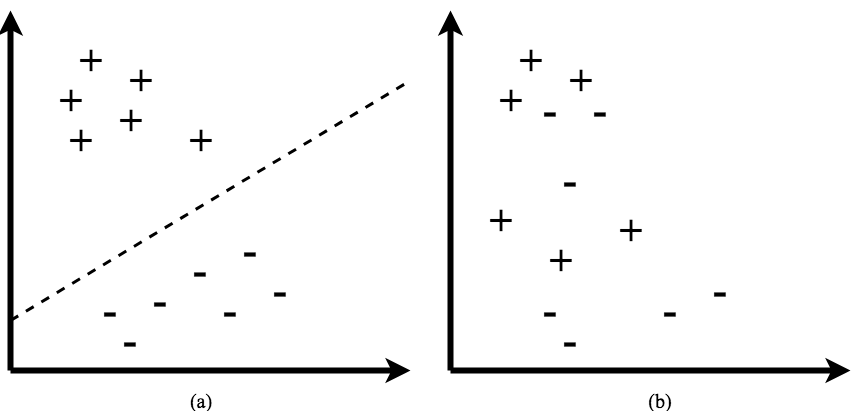
\includegraphics[max width=\textwidth]{separation-surface}
	\caption{A linear decision function (a) can not represent models that can solve more complex problems (b).}
	\label{fig:separation-surface}
\end{figure}

Feed forward networks are trained in the same way as single perceptrons, by running the training dataset through the network and minimizing the error between the outputs and the expected results. Gradient descent is also used to find the approximate weights that will minimize the value of the cost function. However, applying gradient descent to feed forward networks is slightly more involved given the complex nature of the models.\cite{Le15atutorial}.

\begin{figure}[t]
	\centering
	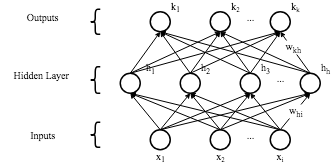
\includegraphics[max width=\textwidth]{feed-forward}
	\caption{A feed forward neural network with a single hidden layer.}
	\label{fig:feed-forward}
\end{figure}

\subsubsection{Backpropagation Algorithm}

The Backpropagation Algorithm is used to apply gradient decent to the individual units of the network\cite{Mitchell}. Initially the network weights are set to random values. Then for each training example, the backpropagation algorithm goes through two stages. First the input is propagated forward and the output $o_u$ of every unit $u$ is calculated. Next comes the backpropagation part where errors are propagated backwards through each layer and new weights are calculated.

For each output unit $k$ an error term $\delta_k$ is calculated
\begin{equation}
\delta_k \leftarrow y_k (1 - y_k)(t_k - y_k)
\end{equation}
where $y_k$ is the actual output of the output unit $k$ and $t_k$ is the target for output unit $k$. Then the error $\delta_h$ for each hidden unit $h$ is calculated
\begin{equation}
\delta_k \leftarrow y_h (1 - y_h) \sum_{k \in outputs} w_{kh} \delta_k
\end{equation}
where $y_h$ is the output from hidden unit $h$ and $w_{kh}$ is the weight of the connection between the hidden unit $h$ and the output unit $k$. Finally the weight of the connection from unit $i$ to unit $j$ is updated using the following update rule
\begin{equation}
w_{ji} \leftarrow w_{ji} + \eta \delta_j x_{ji}
\end{equation}

\subsubsection{Activation Functions}

\begin{figure}[t]
	\centering
	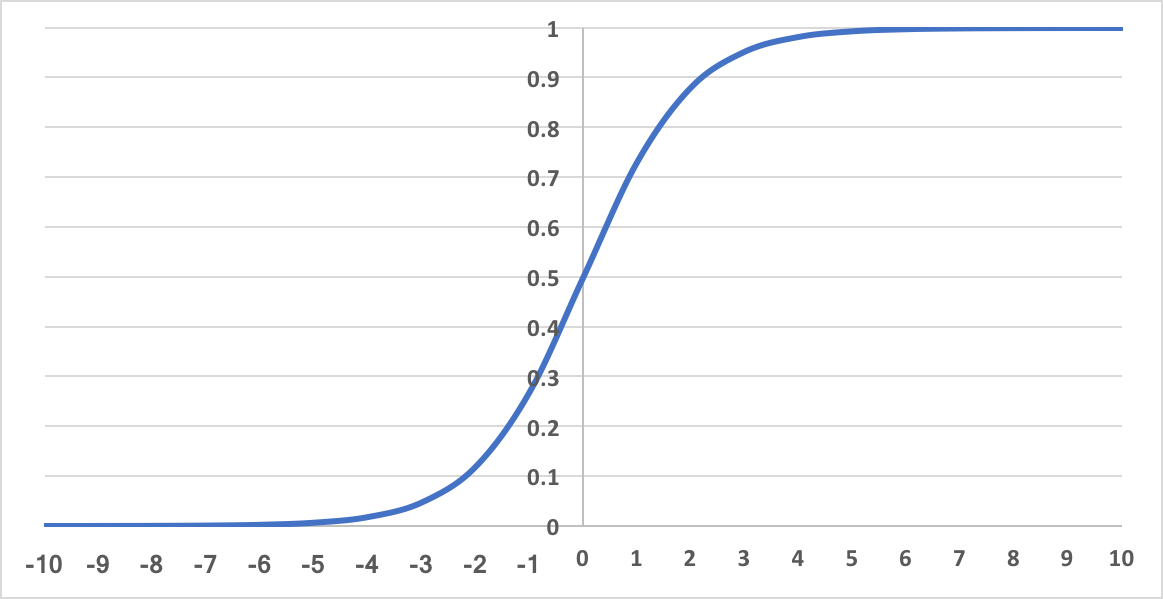
\includegraphics[max width=\textwidth]{sigmoid}
	\caption{A graph depicting the logistic form of the sigmoid function.}
	\label{fig:sigmoid}
\end{figure}

The choice of activation function limits how well the model can represent the underlying problem. In addition, the activation function determines the chain rule that is used to derive the gradient descent update rule. Here we discuss some variations of activation functions and how they affect the ability of neural network models to represent the desired target function. Some functions are best used for output layers because they model a probability distribution like the linear, sigmoid and softmax activations. On the other hand, rectified linear units and hyperbolic tangent activations are used in hidden layers because their derivatives remain generally high. This helps avoid the vanishing gradient problem discussed in Section \ref{sec:background-sequential-models-long-short-term-memory-units}\cite{Goodfellow-et-al-2016}.

Linear units model Gaussian distributions and use a linear activation function where the sum of the weighted inputs is output without transformation. The following formula shows how the output of a linear unit is calculated:
\begin{equation}
\vec{y} = W\vec{x} + b
\end{equation}
Linear activations make it easier for the gradient descent optimizer to find a more desirable minimum. However, they do not represent nonlinear functions very well\cite{Goodfellow-et-al-2016}.

If the output of a neural network involves predicting a binary value, like performing classification with two classes, sigmoid activations can be used. Sigmoid units can be viewed as a linear layer that is then transformed using the sigmoid function\cite{Goodfellow-et-al-2016}. Figure \ref{fig:sigmoid} shows a graph of a sigmoid function and equation \ref{eq:sigmoid} shows the formula for the sigmoid activation function.

The final output activation is known as a softmax activation. These types of units are appropriate for modeling tasks that have an output which is a probability distribution over a discrete variable, for example, a classification problem where the classes are mutually exclusive. Like the sigmoid activation, the softmax activation is a linear layer that is transformed using the softmax function\cite{Goodfellow-et-al-2016}. The following is the softmax function:
\begin{equation}
softmax(z) = \frac{e^z}{\sum{e^z}}
\end{equation}

\begin{figure}[t]
	\centering
	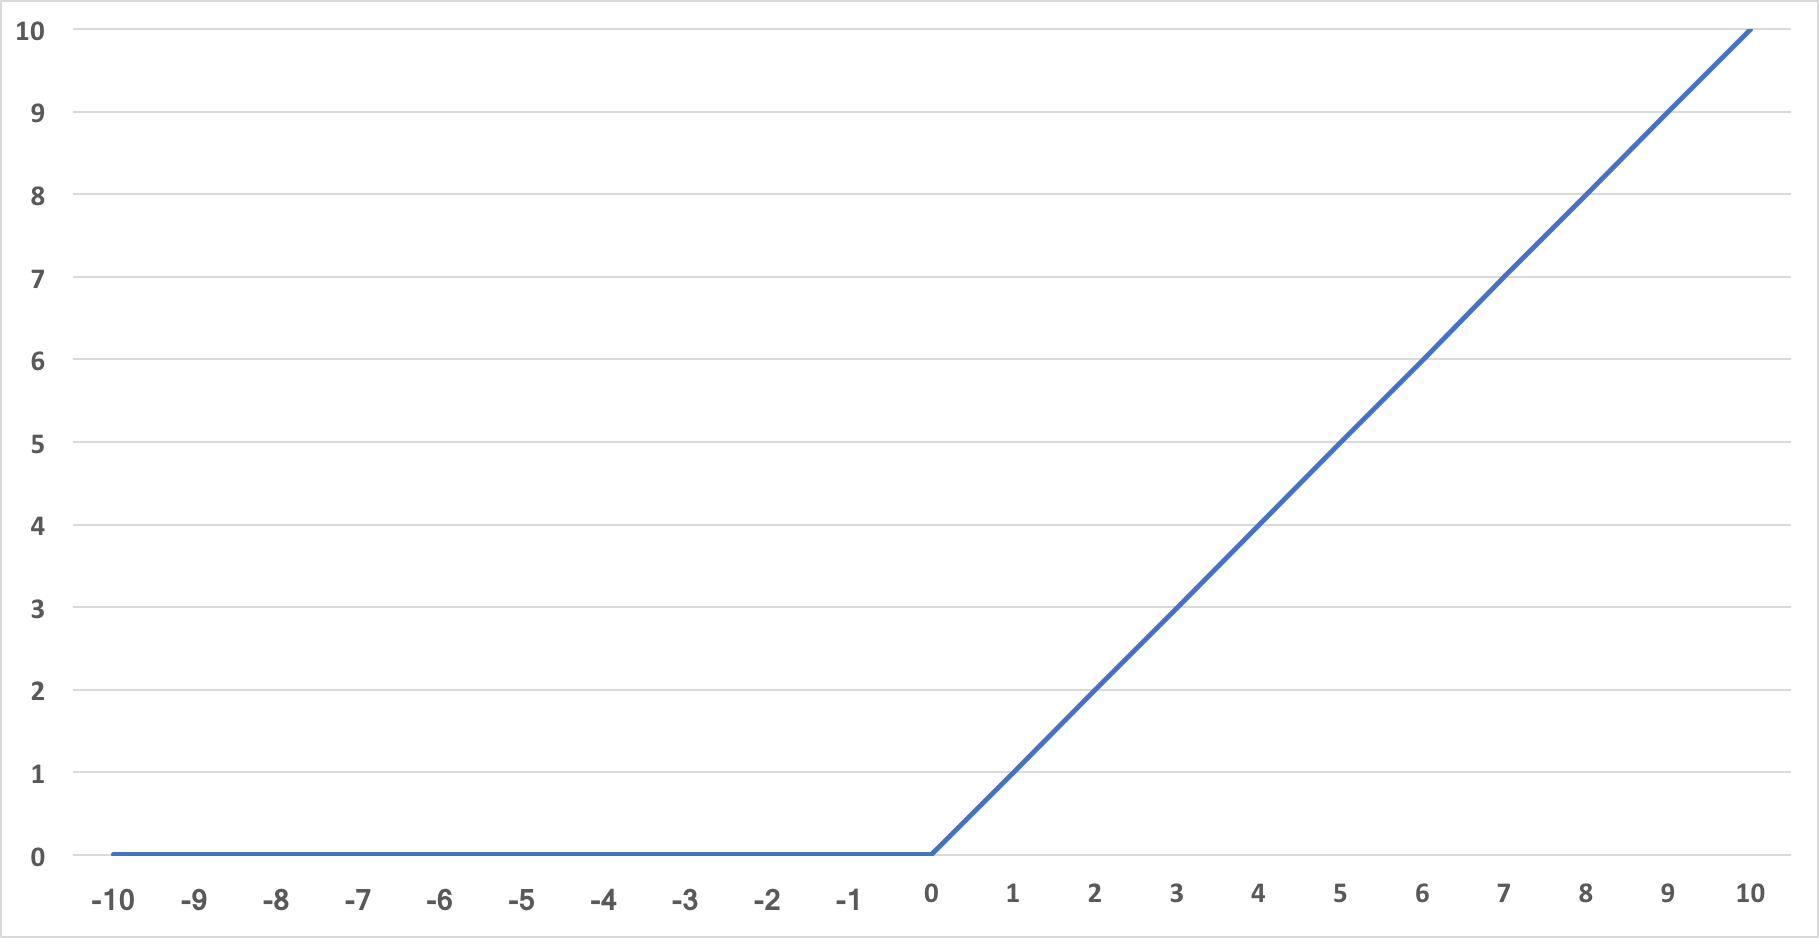
\includegraphics[max width=\textwidth]{relu}
	\caption{A graph of the rectifier function.}
	\label{fig:relu}
\end{figure}

The hyperbolic tangent activation and the rectifier activation are the two most common activation functions in hidden layers. The rectifier is similar to linear activation in that it is easier for gradient descent and also by eliminating values below zero, the gradients remain fairly high which is useful in rapid search for a solution hypothesis \cite{Goodfellow-et-al-2016}. Figure \ref{fig:relu} shows a graph of the rectifier function and the following is the formula for the activation of a rectified linear unit (a neuron with rectifier activation):
\begin{equation}
\label{eq:relu}
y(z) = max\{0, z\}
\end{equation} 

\subsubsection{The Problem of Overfitting}

\begin{figure}[t]
	\centering
	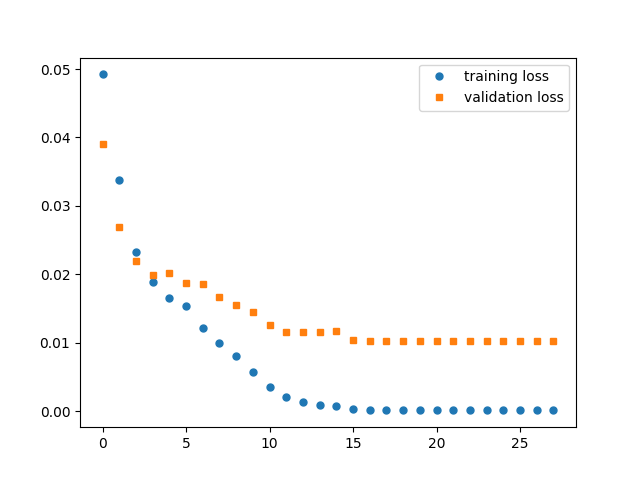
\includegraphics[max width=\textwidth]{overfitting}
	\caption{Comparison of training (circles) and validation (squares) loss over 30 epochs. At the 12th iteration the validation loss stops improving whereas the training loss continues to improve, indicating that the model is starting to overfit.}
	\label{fig:overfitting}
\end{figure}

An important goal of backpropagation is to find a representation that ``fits" the set of training examples and at the same time generalizes to yet unseen data points. Figure \ref{fig:overfitting} shows two graphs that depict the value of the mean squared error against the iteration number of a backpropagation run on a particular dataset. The graph shown in circles shows the errors resulting from the training set and the one in squares shows the errors resulting from the validation set. Notice that the errors from the training set continues to decrease as training proceeds, whereas the errors from the validation set decrease initially but start to stall around the twelfth iteration. This happens because, at the twelfth iteration, the backpropagation algorithm starts to overfit to the training dataset and fails to accurately generalize to the unseen dataset. The weights of the network fit to nuances of the training data that are not representative of the true function. Overfitting is a problem that should be avoided in order for the learning algorithm to create the layers of abstract features that can be used to represent the decision function\cite{Mitchell}.

Using a validation dataset while training is an important mechanism used to prevent backpropagation from overfitting. The validation dataset is independent from the training set and is applied to the model after every epoch. The learning system maintains two copies of the weights of the neural network. One copy holds the weights of the current iteration and the other copy holds the weights of the iteration that performed best on the validation set. When backpropagation stops performing better on the validation set, the best set of weights are returned as the hypothesis learned\cite{Mitchell}.

\subsubsection{K-Fold Cross Validation}

When testing the accuracy of trained neural networks, it is important that the dataset used for testing include a variety of examples that are representative of the overall task. However, with limited datasets, it is difficult to acquire test data that is representative of the problem and therefore it throws into question the effectiveness of the trained model\cite{Goodfellow-et-al-2016}.

Cross-validation is instead used when working with smaller datasets to allow the entire dataset to be used as a test set. With k-fold cross-validation, the dataset is split into k number of non-overlapping subsets. Then training is repeated k times; each time one of the subsets is set aside for testing and the other $k-1$ subsets are used for training. The accuracy score of each iteration is then averaged to produce the overall accuracy of the model. This ensures that the entire dataset contributes to the test set\cite{Goodfellow-et-al-2016}.

In our experiments presented in Chapter 4, we deliberately use small datasets to emulate the difficulty an individual human learner encounters when learning on their own. However, this introduces uncertainty in the accuracy scores obtained from training these models\cite{Goodfellow-et-al-2016}. We therefore use k-fold cross-validation to mitigate this issue.